%                                                                 aa.dem
% AA vers. 9.1, LaTeX class for Astronomy & Astrophysics
% demonstration file
%                                                       (c) EDP Sciences
%-----------------------------------------------------------------------
%
%\documentclass[referee]{aa} % for a referee version
%\documentclass[onecolumn]{aa} % for a paper on 1 column  
%\documentclass[longauth]{aa} % for the long lists of affiliations 
%\documentclass[letter]{aa} % for the letters 
%\documentclass[bibyear]{aa} % if the references are not structured 
%                              according to the author-year natbib style

%
\documentclass{aa}  

%
\usepackage{graphicx}
\usepackage{float}
%%%%%%%%%%%%%%%%%%%%%%%%%%%%%%%%%%%%%%%%
\usepackage{txfonts}
%%%%%%%%%%%%%%%%%%%%%%%%%%%%%%%%%%%%%%%%
%\usepackage[options]{hyperref}
% To add links in your PDF file, use the package "hyperref"
% with options according to your LaTeX or PDFLaTeX drivers.
%
\begin{document} 


   \title{Tunable Kernel-Nulling for direct detection of exoplanets}

   \subtitle{1. Calibration and performance}

   \author{V. Foriel\inst{1},
            F. Martinache\inst{1},
            D. Mary\inst{1}
            \and
            R. Laugier\inst{2}
          }

   \institute{Université Côte d’Azur, Observatoire de la Côte d’Azur Nice, CNRS, Laboratoire Lagrange, Nice, France
         \and
            KU Leuven university, Leuven, Belgium
             }

   \date{Received ---; accepted ---}

% \abstract{}{}{}{}{} 
% 5 {} token are mandatory
 
  \abstract
  % context heading (optional)
  % {} leave it empty if necessary  
   {Lorem ipsum}
  % aims heading (mandatory)
   {Lorem ipsum}
  % methods heading (mandatory)
   {Lorem ipsum}
  % results heading (mandatory)
   {Lorem ipsum}
  % conclusions heading (optional), leave it empty if necessary 
   {Lorem ipsum}

   \keywords{Lorem ipsum}

   \maketitle
%
%-------------------------------------------------------------------

\section{Introduction}

    \begin{enumerate}
        \item Nulling interferometry
        \item Kernel nulling
        \item Integrated optics \& phase shifters
    \end{enumerate}

%--------------------------------------------------------------------

\section{Materials and methods}

    \begin{enumerate}
        \item VLTI/ASGARD (/NOTT?)
        \item Integrated optics \& phase shifters
        \item Studied architecture
        \item Observation conditions (Vegga-like star, noise etc.)
        \item Calibration methods (Fig \ref{fig:perturbed_phases} \& \ref{fig:calibrated_phases})
        \subitem Genertic Algorithm
        \subitem Input obstruction
        \subitem Machine Leaning?
    \end{enumerate}

    \begin{figure}[H]
        \begin{center}
        \begin{tabular}{c}
        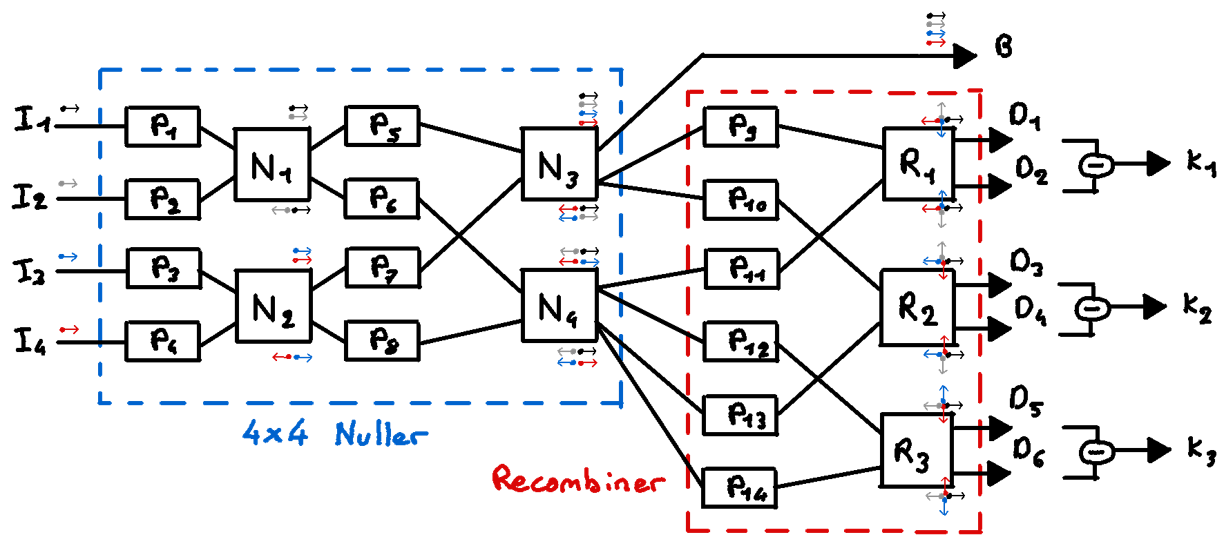
\includegraphics[height=3.5cm]{img/scheme.png}
        \end{tabular}
        \end{center}
        \caption[architecture] 
        { \label{fig:architecture} 
        Studied architecture}
    \end{figure}

    \begin{figure}[H]
        \begin{center}
        \begin{tabular}{c}
        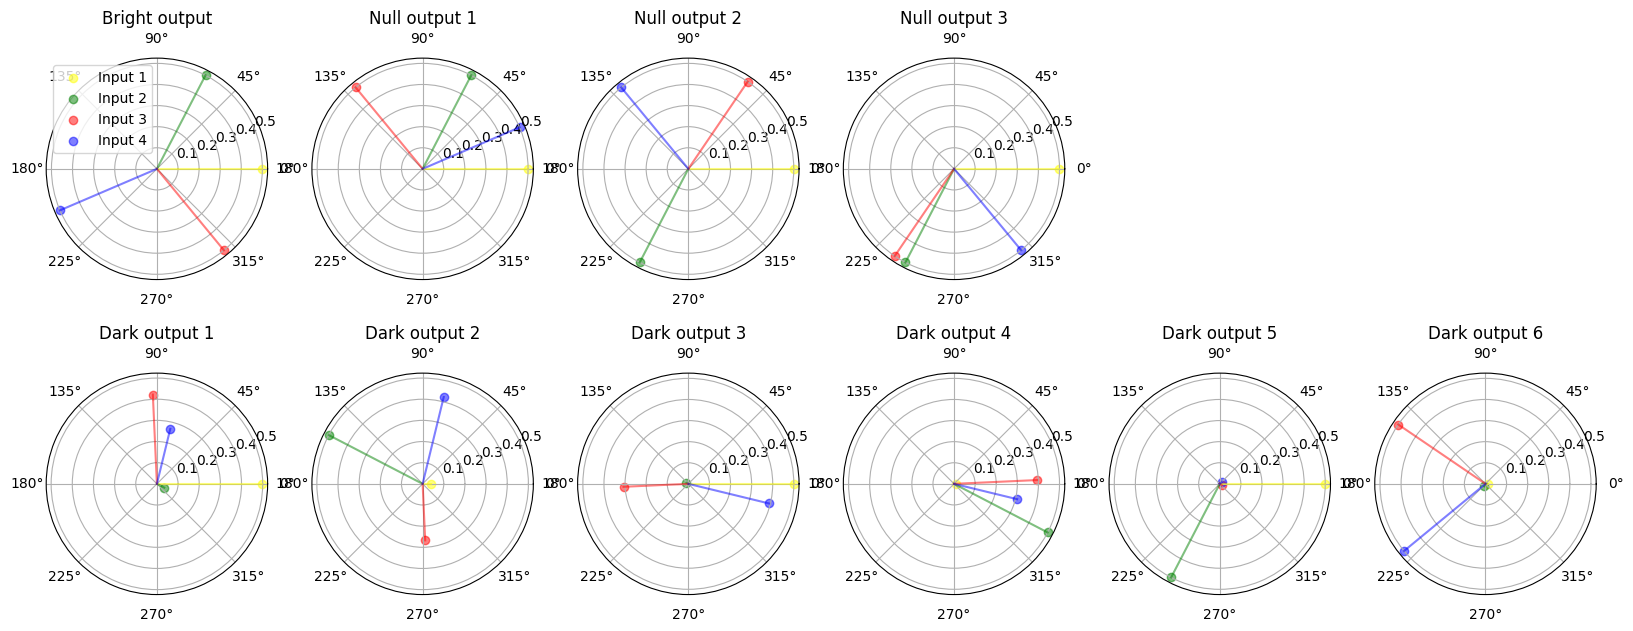
\includegraphics[height=3.2cm]{img/perturbed_phases.png}
        \end{tabular}
        \end{center}
        \caption[perturbed_phases] 
        { \label{fig:perturbed_phases} 
        Perturbed phases}
    \end{figure}

    \begin{figure}[H]
        \begin{center}
        \begin{tabular}{c}
        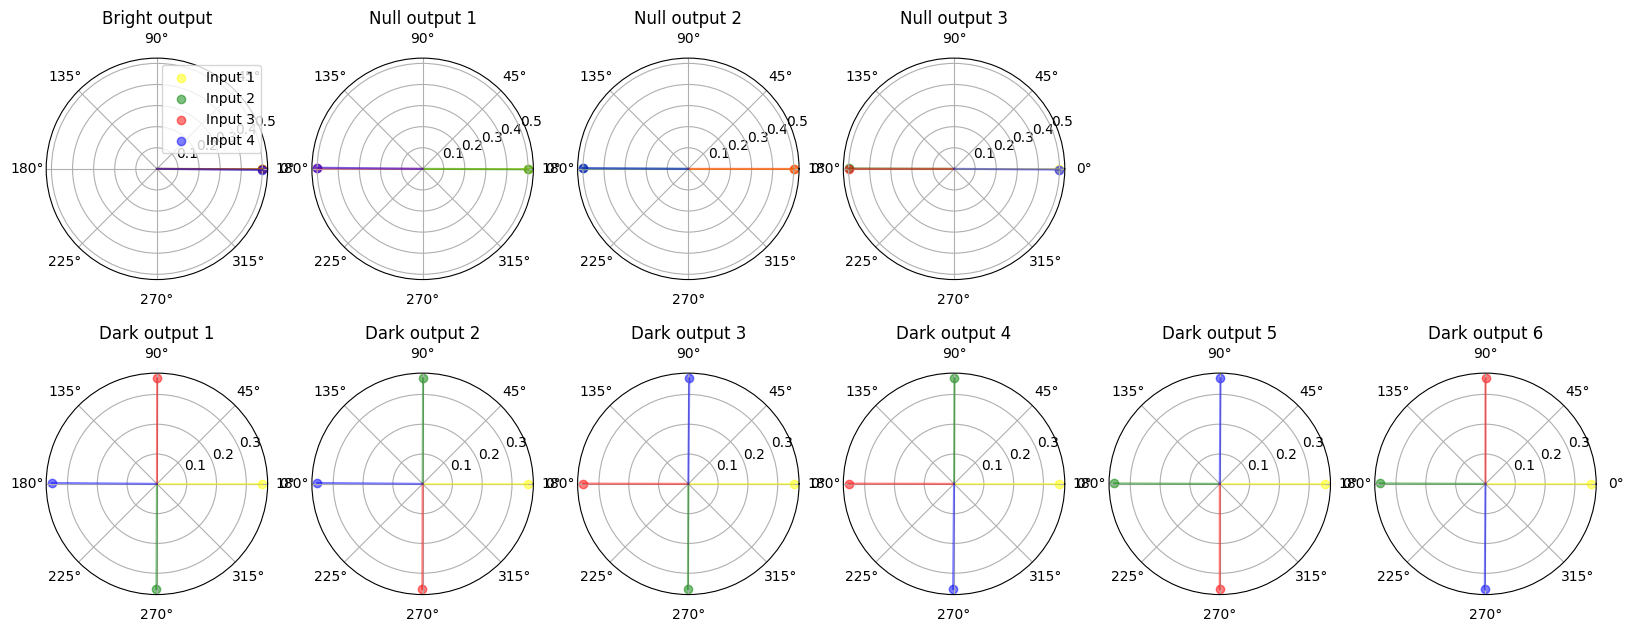
\includegraphics[height=3.2cm]{img/calibrated_phases.png}
        \end{tabular}
        \end{center}
        \caption[calibrated_phases] 
        { \label{fig:calibrated_phases} 
        Calibrated phases}
    \end{figure}

%--------------------------------------------------------------------

\section{Results and limitations}

    \begin{enumerate}
        \item Numerical results
        \subitem Kernel-Null depth (Fig \ref{fig:calibration_genetic} \& \ref{fig:calibration_obstruction})
        \subitem Kernel inversion and swapping 
        \item Laboratory results
        \item Laboratory limitations (ex. crosstalk)
    \end{enumerate}

    \begin{figure}[H]
        \begin{center}
        \begin{tabular}{c}
        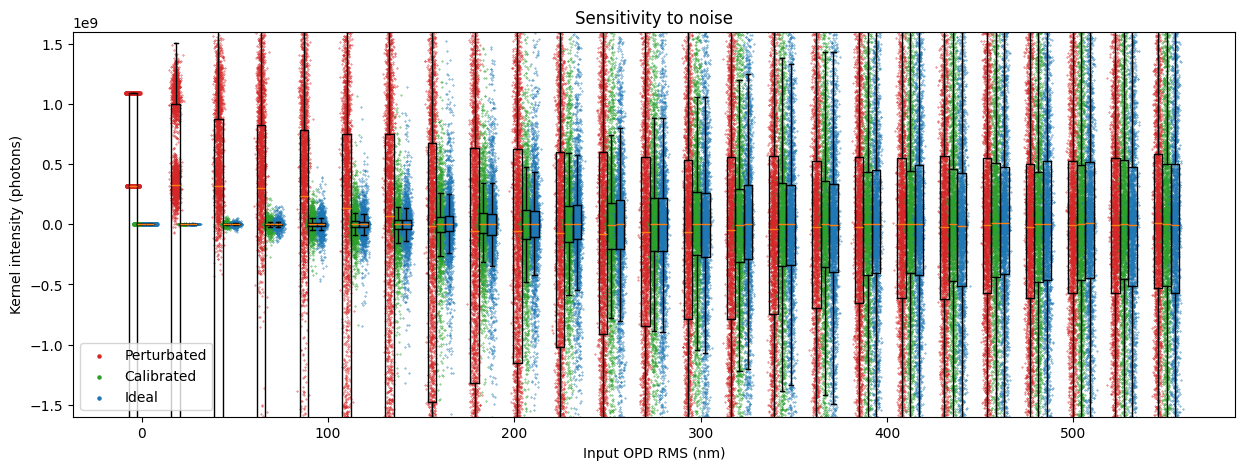
\includegraphics[height=3cm]{img/noise_sensitivity.png}
        \end{tabular}
        \end{center}
        \caption[noise_sensitivity] 
        { \label{fig:noise_sensitivity} 
        Sensitivity to input noise}
    \end{figure}

    \begin{figure}[H]
        \begin{center}
        \begin{tabular}{c}
        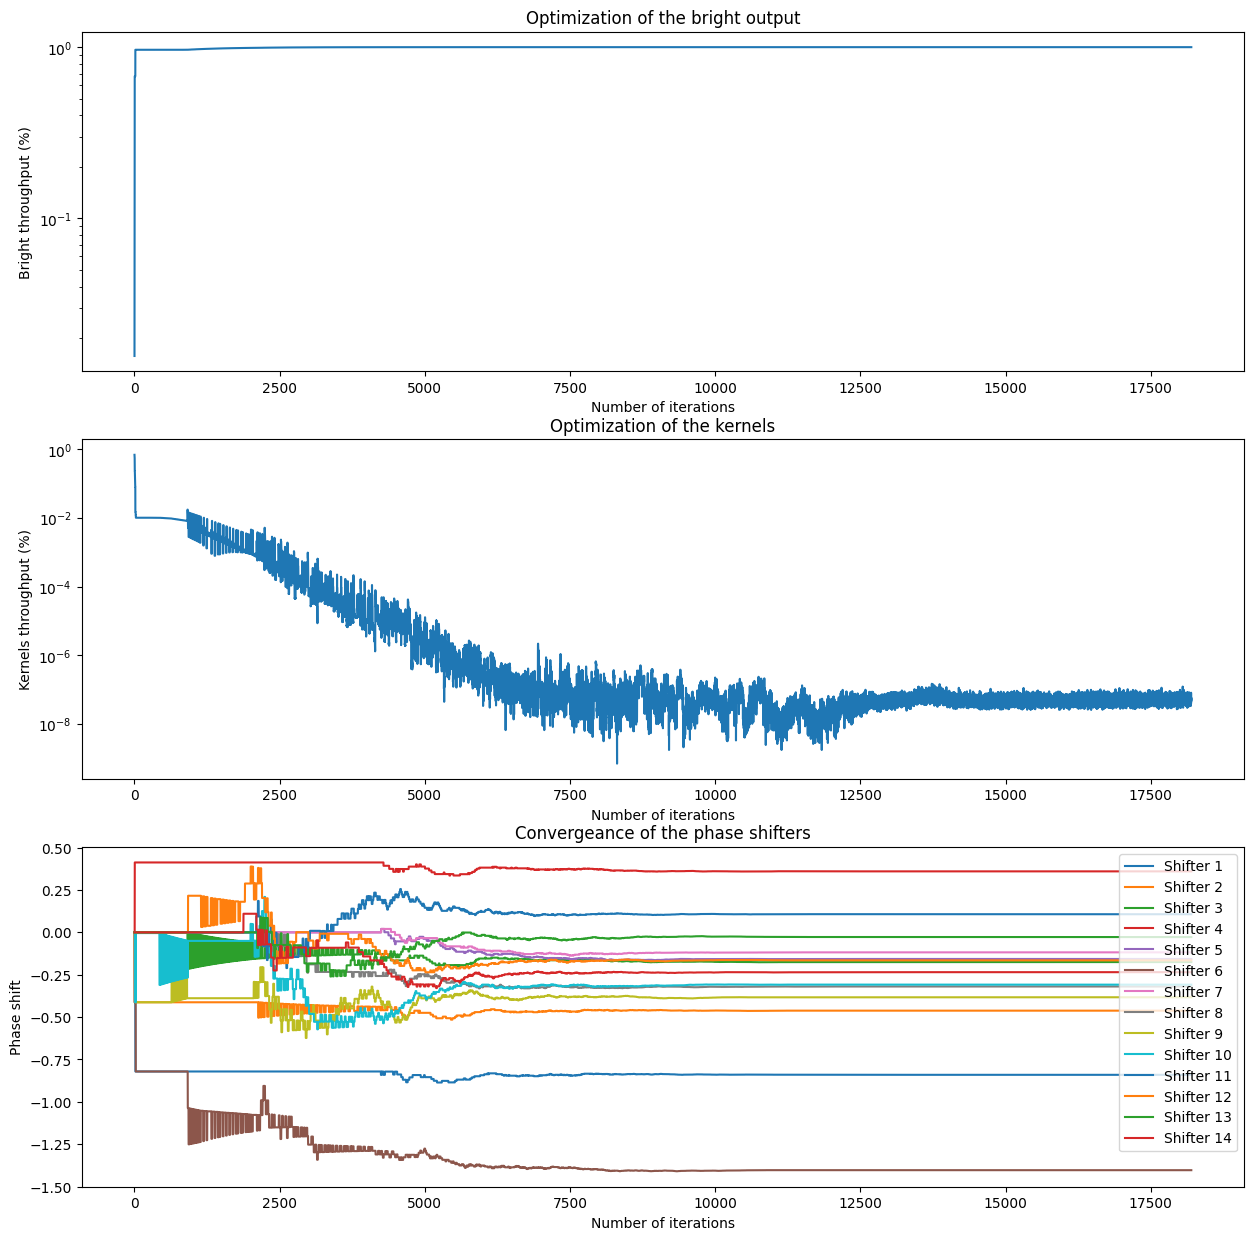
\includegraphics[height=7cm]{img/calibration_genetic.png}
        \end{tabular}
        \end{center}
        \caption[calibration_genetic] 
        { \label{fig:calibration_genetic} 
        Calibration using genetic algorithm}
    \end{figure}

    \begin{figure}[H]
        \begin{center}
        \begin{tabular}{c}
        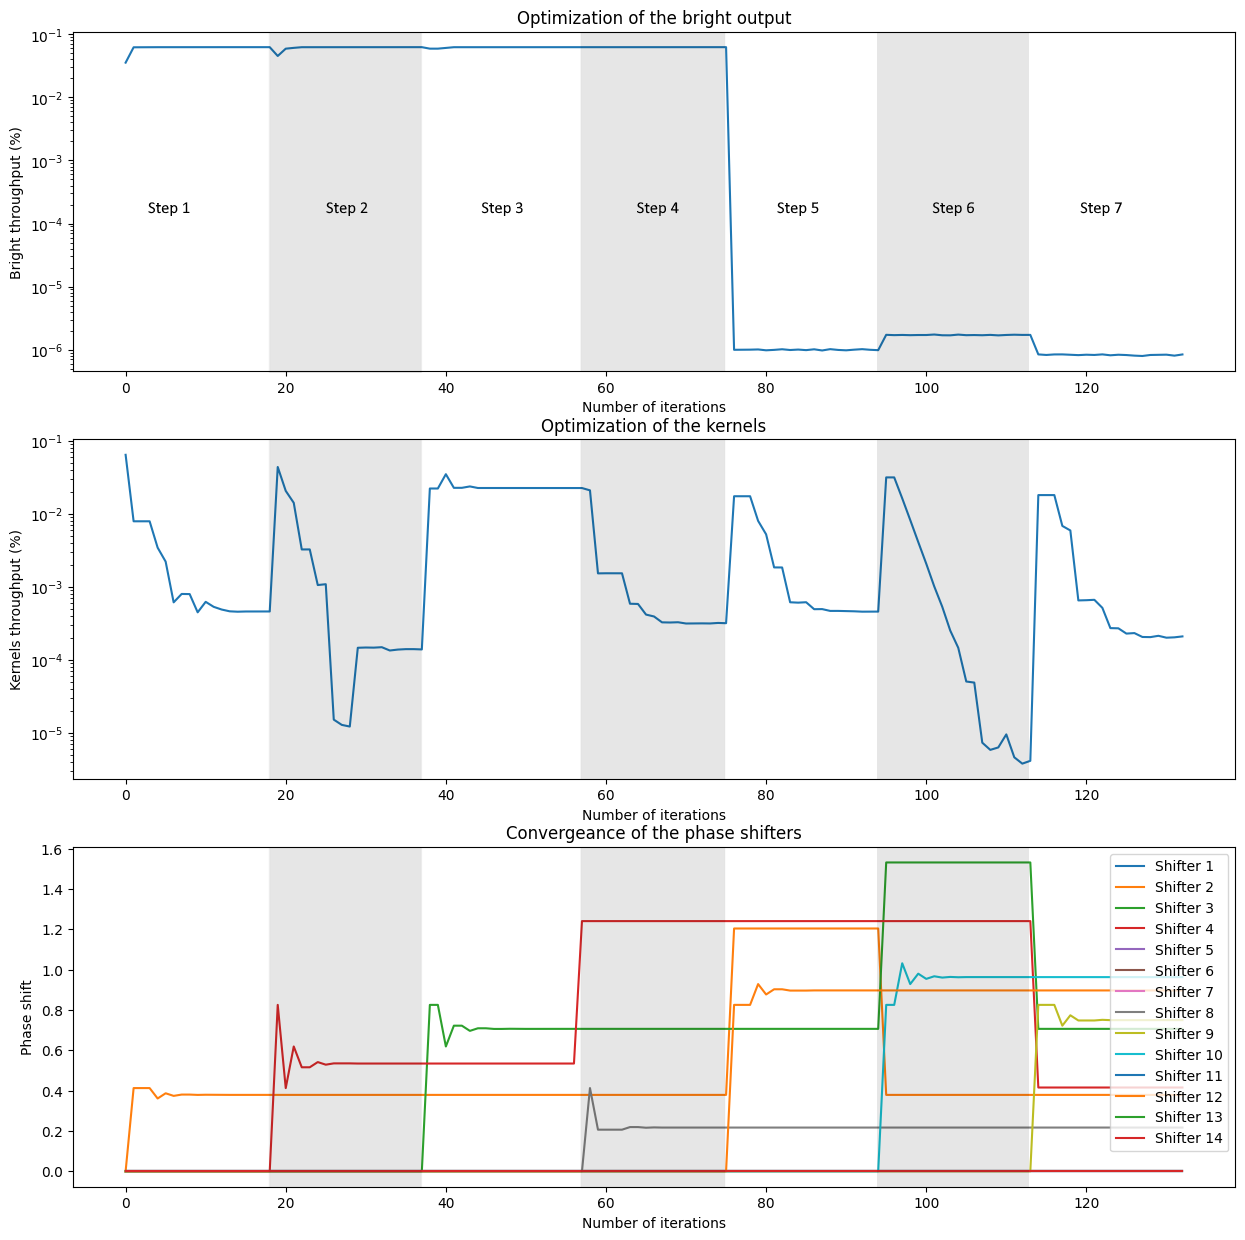
\includegraphics[height=7cm]{img/calibration_obstruction.png}
        \end{tabular}
        \end{center}
        \caption[calibration_obstruction] 
        { \label{fig:calibration_obstruction} 
        Calibration using input obstruction}
    \end{figure}

%-----------------------------------------------------------------

\section{Conclusions and prospects}

   \begin{enumerate}
      \item Conditions for noticing a performance gain
      \item Need of a post calibration caracterization process to identify the outputs
      \item Deeper statistical analysis is required to truely caracterize performance gain (the null depth is not the only relevant parameter)
      \item Architecture limitations (ex. no amplitude modulation, no photometric outputs)
   \end{enumerate}

\begin{acknowledgements}
      Lorem ipsum
\end{acknowledgements}

% WARNING
%-------------------------------------------------------------------
% Please note that we have included the references to the file aa.dem in
% order to compile it, but we ask you to:
%
% - use BibTeX with the regular commands:
%   \bibliographystyle{aa} % style aa.bst
%   \bibliography{Yourfile} % your references Yourfile.bib
%
% - join the .bib files when you upload your source files
%-------------------------------------------------------------------

\begin{thebibliography}{}

  \bibitem{lorem ipsum} Lorem ipsum

\end{thebibliography}

\end{document}
